\documentclass[11pt]{article}

\usepackage{amsmath,amsthm,amssymb}

%%%%% Matrix stretcher
% use it as:
%\begin{pmatrix}[1.5]
% ...
\makeatletter
\renewcommand*\env@matrix[1][\arraystretch]{%
  \edef\arraystretch{#1}%
  \hskip -\arraycolsep
  \let\@ifnextchar\new@ifnextchar
  \array{*\c@MaxMatrixCols c}}
\makeatother
%%%%%%%%%%%%%%%%%%%%%%%%%%

\newcommand\extrafootertext[1]{%
    \bgroup
    \renewcommand\thefootnote{\fnsymbol{footnote}}%
    \renewcommand\thempfootnote{\fnsymbol{mpfootnote}}%
    \footnotetext[0]{#1}%
    \egroup
}


%%%%%%%%%%%%% Colors %%%%%%%%%%%%%
\usepackage[dvipsnames]{xcolor}

\definecolor{C0}{HTML}{1d1d1d}
\definecolor{C1}{HTML}{1e3668}
\definecolor{C2}{HTML}{199d8b}
\definecolor{C3}{HTML}{d52f4c}
\definecolor{C4}{HTML}{5ab2d6}
\definecolor{C5}{HTML}{ffb268}
\definecolor{C6}{HTML}{ff7300} % for commenting - {fire orange}dd571c
\definecolor{C7}{HTML}{777b7e} % for remarks - {steel grey}
\color{C0}
%%%%%%%%%%%%%%%%%%%%%%%%%%%%%%%%



%%%%%%%%%%%%% Fonts %%%%%%%%%%%%% 
%\usepackage{fontspec}
\usepackage[no-math]{fontspec} % for text

\emergencystretch=8pt
\hyphenpenalty=1000 % default 50
\tolerance=800      % default 200
%\righthyphenmin=4
%\lefthyphenmin=4

%%% Text Font: Vollkorn + Math Font: Latin Modern (default) %%%
\setmainfont{Vollkorn}[
UprightFont = Vollkorn-Regular,
ItalicFont =Vollkorn-Italic, 
BoldItalicFont={Vollkorn-BoldItalic},
BoldFont = Vollkorn-Bold,
RawFeature=+lnum,
WordSpace=1.7,
] 

%%% We need this for math font packages other than latin modern %%%
% \usepackage{unicode-math}        % for math

%%% Text Font: Palatino + Math Font: Asana-Math %%%
%\setmainfont{Palatino}[
%BoldFont = Palatino-Bold,
%ItalicFont = Palatino-Italic,
%BoldItalicFont={Palatino-BoldItalic},
%RawFeature=+lnum,
%WordSpace=1.7,
%]
%\setmathfont{asana-math}

%%% Text Font: Arno Pro + Math Font: Minion Pro %%%
%\setmainfont{Arno Pro}[
%UprightFont = *-Regular,
%ItalicFont = Vollkorn-Italic, 
%BoldItalicFont={*-BoldItalic},
%BoldFont = *-Bold,
%RawFeature=+lnum,
%WordSpace=1.7,
%Scale= 1.1
%] 
% Minion Pro is too expensive

%%% Math Fonts %%%
%\setmathfont{Vollkorn}
%\setmathfont{Latin Modern Math}
%\setmathfont{TeX Gyre Pagella Math}
%\setmathfont{TeX Gyre Termes Math}
%\setmathfont{TeX Gyre DejaVu Math}
%\setmathfont[Scale=MatchLowercase]{DejaVu Math TeX Gyre}
%\setmathfont{XITS Math}
%\setmathfont{Libertinus Math}
%\setmathfont[Scale=MatchUppercase]{Asana Math}
%\setmathfont{STIX Two Math}

%\usepackage{kpfonts-otf}
%\setmathfont{KpMath-Regular.otf}[version=regular]
%\setmathfont{KpMath-Bold.otf}[version=bold]
%\setmathfont{KpMath-Semibold.otf}[version=semibold]
%\setmathfont{KpMath-Sans.otf}[version=sans]
%\setmathfont{KpMath-Light.otf}[version=light]


%%% CJK Fonts %%%
\usepackage[scale=.78]{luatexja-fontspec}
\setmainjfont{BabelStone Han}[AutoFakeBold]
%%%%%%%%%%%%%%%%%%%%%%%%%%%%%%%


% This package simplifies the insertion of external multi-page PDF or PS documents.
\usepackage{pdfpages}

% cref
\usepackage{hyperref}
\hypersetup{
    colorlinks=true,
    linkcolor=C4,
    filecolor=magenta,      
    urlcolor=cyan,
    }

\usepackage[nameinlink,noabbrev,capitalize]{cleveref}
% \crefname{ineq}{}{}
% \crefname{equation}{}{}
% \creflabelformat{ineq}{#2{\textup{(1)}}#3}
% \creflabelformat{equation}{#2\textup{(#1)}#3}

%%%%%%%%%%%%% Environments %%%%%%%%%%%%%%%%
%amsthm has three separate predefined styles:	
%
%\theoremstyle{plain} is the default. it sets the text in italic and adds extra space above and below the \newtheorems listed below it in the input. it is recommended for theorems, corollaries, lemmas, propositions, conjectures, criteria, and (possibly; depends on the subject area) algorithms.
%
%\theoremstyle{definition} adds extra space above and below, but sets the text in roman. it is recommended for definitions, conditions, problems, and examples; i've alse seen it used for exercises.
%
%\theoremstyle{remark} is set in roman, with no additional space above or below. it is recommended for remarks, notes, notation, claims, summaries, acknowledgments, cases, and conclusions.

%%%  theorem-like environment %%%
\theoremstyle{plain} % default theorem style
\newtheorem{theorem}{Theorem}[section]
\newtheorem{assumption}[theorem]{Assumption}
\newtheorem{lemma}[theorem]{Lemma}
\newtheorem{corollary}[theorem]{Corollary}
\newtheorem{proposition}[theorem]{Proposition}
\newtheorem{property}[theorem]{Property}

\newtheorem{definition}[theorem]{Definition}

%%% definition-like environment %%%
%\theoremstyle{definition}
\newtheorem{example}[theorem]{Example}
\newtheorem{problem}[theorem]{Problem}


%%% framed package is great %%%
\usepackage{framed}
\newenvironment{solution}
{\color{C2}\normalfont\begin{framed}\begingroup\textbf{Solution:} }
  {\endgroup\end{framed}}
  
\newenvironment{topic}
{\color{C2}\normalfont\begin{framed}\begingroup }
  {\endgroup\end{framed}}
  
\newtheoremstyle{remark}% name of the style to be used
  {}% measure of space to leave above the theorem. E.g.: 3pt
  {}% measure of space to leave below the theorem. E.g.: 3pt
  {\color{C3}}% name of font to use in the body of the theorem
  {}% measure of space to indent
  {\color{C3}\bfseries}% name of head font
  {.}% punctuation between head and body
  { }% space after theorem head; " " = normal interword space
  {}
\theoremstyle{remark}
\newtheorem{remarkx}[theorem]{Remark}
\newenvironment{remark}
  {\pushQED{\qed}\renewcommand{\qedsymbol}{$\triangle$}\remarkx}
  {\popQED\endremarkx}
  
\newenvironment{point}
  {\O~~}
  {}

\usepackage{thmtools}
\usepackage{thm-restate}
%%%%%%%%%%%%%%%%%%%%%%%%%%%%%%%%%%%%


% This package is for the long equal sign \xlongequal{}
\usepackage{extarrows}

%%%%%%%%%%%% Algorithms %%%%%%%%%%%%
\usepackage{etoolbox} 
\usepackage{setspace}
\usepackage{algorithm}
\AtBeginEnvironment{algorithmic}{\onehalfspacing}
\usepackage{algorithmicx}
\usepackage[noend]{algpseudocode}

\algrenewcommand\algorithmicindent{1.0em}
\let\Algorithm\algorithm
\renewcommand\algorithm[1][]{\Algorithm[#1]}%\fontsize{11}{16}\selectfont}

\newenvironment{labelalgorithm}[4][t]{%
\begin{algorithm}[#1]
%\newcommand{\thealgorithmlabel}{#2}
\newcommand{\thealgorithmname}{#3}
%\newcommand{\thealgorithmcap}{#4}
\customlabel{alg:name:#2}{\textproc{#3}}
%\customlabel{alg:cap:#2}{#4}
\caption{#4}\label{alg:#2}
}{\end{algorithm}}


\makeatletter
\newcommand{\customlabel}[2]{%
   \protected@write \@auxout {}{\string \newlabel {#1}{{#2}{\thepage}{#2}{#1}{}} }%
   \hypertarget{#1}{}%
}
\makeatother


%\algdef{SE}[FUNCTION]{Procedure}{EndProcedure}%
%   [2]{\algorithmicclass\ \textproc{#1}\ifthenelse{\equal{#2}{}}{}{$($#2$)$}}%
%   {\algorithmicend\ \algorithmicclass}%

\algnewcommand\algorithmicclass{\textbf{class}}
\algdef{SE}[FUNCTION]{Class}{EndClass}%
   [2]{\algorithmicclass\ \textproc{#1}\ifthenelse{\equal{#2}{}}{}{$($#2$)$}}%
   {\algorithmicend\ \algorithmicclass}%

% Tells algorithmicx not to print an empty line if `noend' is set 
\makeatletter
\ifthenelse{\equal{\ALG@noend}{t}}%
  {\algtext*{EndClass}}
  {}%
\makeatother
%%%%%%%%%%%%%%%%%%%%%%%%%%%%%%%%%%%%


% Page Formatting
\usepackage[
    paper=a3paper,
    inner=22mm,         % Inner margin
    outer=22mm,         % Outer margin
    bindingoffset=0mm, % Binding offset
    top=28mm,           % Top margin
    bottom=22mm,        % Bottom margin
    %showframe,         % show how the type block is set on the page
]{geometry}

\setlength{\parindent}{0em}
\setlength{\parskip}{.7em}


\usepackage{tikz}
\usepackage{graphicx}
\usepackage{subcaption} % for subplots
\usepackage{multicol}   % for multicolumns
\usepackage{wrapfig}    % for inserting figures in multicolumns
\usepackage{enumitem}
\setlist{topsep=0pt}

\usepackage{bm}

\usepackage[font=scriptsize,labelfont=bf]{caption}
\usepackage{listings}
\lstset{basicstyle=\ttfamily,breaklines=true}
% \setlength{\parskip}{1em}
% \setlength{\parindent}{0em}
\usepackage{dsfont}
\newcommand{\bOne}{\mathds{1}}
\newcommand{\PP}{\mathbb{P}}
\newcommand{\EE}{\mathbb{E}}
\newcommand{\VV}{\mathbb{V}}
\newcommand{\CoV}{\operatorname{Co\mathbb{V}}}

% header
\usepackage{fancyhdr}
\pagestyle{fancy}
\fancyhead{}
\fancyhead[L]{\small   \bfseries Notes}
\fancyhead[C]{\small   \bfseries Fall 2023}
\fancyhead[R]{\small   \bfseries Zhou}


\begin{document}

\begin{center}
  \text{\Large{Reinforcement Learning
    }}

  {\text{Kaiwen Zhou}}
\end{center}
\vspace{2em}

\tableofcontents

%%%%%%%%%%%%%%%%%%%%%%%%%%%%%%%%%%%%%%%%%%%%%%%%
\section{Topic: Markov Decision Processes}
MDPs are a classical formalization of sequential decision making, where actions
influence not just immediate rewards, but also subsequent situations, or states,
and through those future rewards. Thus MDPs involve delayed reward and the need
to trade off immediate and delayed reward.

%%%%%%%%%%%%%%%%%%%%%%%%%
\subsection{Introduction}
MDPs are a classical formalization of sequential decision making, where
actions influence not just immediate rewards, but also subsequent situations,
or states, and through those future rewards. Thus MDPs involve delayed reward and the need to trade off immediate and
delayed reward. A Markov decision process contains, in particular, a Markov process for
a variable that is called the state. If you have ever encountered the concept of a Markov chain described by
a transition probability matrix, then you are already familiar with the
concept. Similarly, if you have ever used a Kalman filter, you have worked with
continuous Markov processes whose probability transition "matrix" is instead a
Gaussian density. MDPs are meant to be a straightforward framing of the problem of
learning from interaction to achieve a goal. The learner and decision maker is called the agent. The thing it interacts with, comprising everything outside the agent, is
called the environment. These interact at each of a sequence of discrete time steps $t=0,1,2,
  \ldots$, the agent selecting actions and the environment responding to these
actions and presenting new situations to the agent. The environment also gives rise to rewards, special numerical values
that the agent seeks to maximize over time through its choice of actions.

\begin{figure}[!htp]
  \centering
  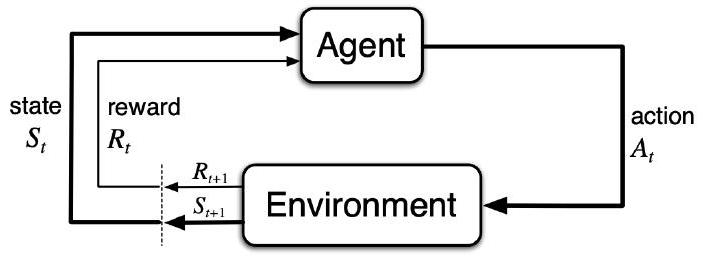
\includegraphics[width=0.3\textwidth]{images/2023_12_18_21a3a2e71c8a014fc272g-05}
  \caption{Markov Decision Processes}
  \label{fig:MDP}
\end{figure}

At each time step $t$, the agent receives some representation of the
environment's state, $S_{t} \in \mathcal{S}$, and on that basis selects an
action, $A_{t} \in \mathcal{A}(s)$. One time step later, in part as a consequence of its action, the agent
receives a numerical reward,

$$
  R_{t+1} \in \mathcal{R} \subset \mathbb{R}
$$

and finds itself in a new state, $S_{t+1}$.

The way that the agent selects actions is called a policy. Although it is not a particularly clever one, we want to allow as one
valid policy, that the agent will roll some combination of dice and/or flip
various coins to arrive at the chosen action. In other words a policy may explicitly involve randomness in the choice. Formally, a policy is a mapping from states to a vector of probabilities
of selecting each possible action. If the agent is following policy $\pi$ at time $t$, then

$$
  \pi(a \mid s)
$$

is the probability that $A_{t}=a$, given that $S_{t}=s$.

Any randomness influencing the action choice is independent of the
randomness influencing the state-transition dynamics. In a finite MDP, the sets of states, actions, and rewards

$$
  \mathcal{S}, \mathcal{A}, \text { and } \mathcal{R}
$$

all have a finite number of elements.

In this case, the random variables $R_{t}$ and $S_{t}$ have well defined
discrete probability distributions

$$
  p\left(s^{\prime}, r \mid s, a\right)
$$

dependent only on the preceding state and action:

$$
  p\left(s^{\prime}, r \mid s, a\right)=\operatorname{prob}\left(S_{t}=s^{\prime}, R_{t}=r \mid S_{t-1}=s, A_{t-1}=a .\right)
$$

The probability function $p$ defines the dynamics of the MDP. In a Markov decision process, the probability of each possible value for
the state and the reward,

$$
  S_{t} \text { and } R_{t} \text {, }
$$

depends on the immediately preceding state and action,

$$
  S_{t-1} \text { and } A_{t-1} \text {, }
$$

and, given the preceding state and action, it depends not at all on earlier
states and actions.  The state must include information about all aspects of the past
agent-environment interaction that make a difference for the future. From the four-argument dynamics function, $p$, one can (in principle, if
there are not too many states) compute anything else one might want to know
about the environment, such as the state-transition probabilities

$$
  p\left(s^{\prime} \mid s, a\right)=\sum_{r \in \mathcal{R}} p\left(s^{\prime}, r \mid s, a\right)
$$

We can also compute the expected rewards for state-action pairs as

$$
  \mathbb{E}\left[R_{t} \mid S_{t-1}=s, A_{t-1}=a\right]=\sum_{r \in \mathcal{R}} r \sum_{s^{\prime} \in \mathcal{S}} p\left(s^{\prime}, r \mid s, a\right)
$$

and the expected rewards for state-action-nextstate triples, etc.

\subsection{Goals and Rewards}
The use of a reward signal to formalize the idea of a goal is one of the
most distinctive features of reinforcement learning. Although formulating goals in terms of reward signals might at first
appear limiting, in practice it has proved to be flexible and widely
applicable. In making a robot learn how to escape from a maze, the reward is often
-1 for every time step that passes prior to escape; this encourages the agent
to escape as quickly as possible. It is critical that the rewards we set up truly indicate what we want
accomplished. For example, a chess-playing agent should be rewarded only for actually
winning, not for achieving subgoals such as taking its opponent's pieces or
gaining control of the center of the board. If achieving these subgoals were rewarded, then the agent might find a
way to achieve them without achieving the real goal; it might find a way to
take the opponent's pieces at the cost of losing the game.


\subsection{Episodes}
In general, we seek to maximize the expected return, where the return,
denoted $G_{t}$, is defined as some specific function of the reward sequence. In the simplest case the return is the sum of the rewards:

$$
  G_{t}=R_{t+1}+R_{t+2}+\cdots+R_{T}
$$

where $T$ is a final time step.

This approach makes sense in applications in which there is a natural
notion of final time step, that is, when the agent-environment interaction
breaks naturally into subsequences, which we call episodes. Episodes could be plays of a game, trips through a maze, and many other
types of sequential play. Each episode ends in a special state called the terminal state, followed
by a reset to a standard starting state or to a sample from a standard
distribution of starting states. Even if you think of episodes as ending in different ways, such as
winning and losing a game, the next episode begins independently of how the
previous one ended. Thus the episodes can all be considered to end in the same terminal
state, with different rewards for the different outcomes. The time of termination, $T$, is a random variable that normally varies
from episode to episode. On the other hand, in many cases the agent-environment interaction does
not break naturally into identifiable episodes, but goes on continually
without limit.

For example, this would be the natural way to formulate an on-going
process-control task, or an application to a robot with a long life span. We call these continuing tasks. The formulation (10.1) is problematic for continuing tasks, because
there is no natural $T$.

In continuing tasks we often instead define

$$
  G_{t}=\sum_{k=0}^{\infty} \gamma^{k} R_{t+1+k}, \quad \text { for } \quad 0<\gamma<1
$$

The discount rate determines the present value of future rewards. If

$$
  0<\gamma<1
$$

the infinite sum (10.2) has a finite value as long as the reward sequence

$$
  \left\{R_{k}\right\}
$$

is bounded.

Note the useful identity

$$
  G_{t}=R_{t+1}+\gamma G_{t+1}
$$

which follows directly from the definition.

In fact, there is a way to consider episodic tasks as a special kind of
continuing task, which would allow us to work in a unified mathematical
notation and framework. We have defined the return as a sum over a finite number of terms in one
case (10.1) and as a sum over an infinite number of terms in the other (10.2). These two can be unified by considering episode termination to be the
entering of a special absorbing state that transitions only to itself and that
generates only rewards of zero. For example, suppose that on a particular run, we get the reward
sequence

$$
  +1,+1,+1,0,0,0, \ldots
$$

Summing these, we get the same return whether we sum over the first $T$
rewards (here $T=3$) or over the full infinite sequence. This remains true even if we introduce discounting. With these conventions, we can use the formulation (10.2):

$$
  G_{t}=\sum_{k=0}^{\infty} \gamma^{k} R_{t+1+k}
$$

for either continuing or episodic tasks.

In a problem where all episodes terminate, we can set

$$
  \gamma=1
$$

without any convergence problems.

\subsection{Value Functions}
The value function of a state $s$ under a policy $\pi$, denoted

$$
  v_{\pi}(s),
$$

is the expected return when starting in $s$ and following policy $\pi$
thereafter.

For MDPs, we can define $v_{\pi}$ by:

$$
  v_{\pi}(s)=\mathbb{E}_{\pi}\left[G_{t} \mid S_{t}=s\right]
$$

where the notation $\mathbb{E}_{\pi}$ means the expectation value in the
probability space associated to always following $\pi$.

Convince yourself that if a materially-different policy were selected,
then the distribution of the random variable $G_{t}$ will typically be
different.

Note that the value of

$$
  \mathbb{E}_{\pi}\left[G_{t} \mid S_{t}=s\right]
$$

appears superficially to depend on $t$, but in actual fact it is independent of
$t$ due to stationarity and the Markov property.

Note that the value of the terminal state, if any, is always zero. Similarly, we define $q_{\pi}(s, a)$, as the expected return starting
from $s$, taking the action $a$, and thereafter following policy $\pi$ :

$$
  q_{\pi}(s, a)=\mathbb{E}_{\pi}\left[G_{t} \mid S_{t}=s, A_{t}=a\right]
$$

Now $v_{\pi}(s)$ is called the state-value function and the function

$$
  q_{\pi}(s, a)
$$

is called the action-value function.

The value functions $v_{\pi}$ and $q_{\pi}$ can be estimated from
experience. For example, if an agent follows policy $\pi$ and maintains an average,
for each state encountered, of the actual returns that have followed that
state, then the average will converge to the state's value as the number of
times that state is encountered approaches infinity. If separate averages are kept for each action taken in each state, then
these averages will similarly converge to the action values. Such estimation methods are Monte Carlo methods. A fundamental property of value functions used throughout reinforcement
learning and dynamic programming is that they satisfy recursive relationships
similar to that which we have already established for the return.

For any policy $\pi$ and any state $s$, the following consistency
condition holds:

$$
  \begin{aligned}
    v_{\pi}(s) & =\mathbb{E}_{\pi}\left[G_{t} \mid S_{t}=s\right]                                                                                                                     \\
               & =\mathbb{E}_{\pi}\left[R_{t+1}+\gamma G_{t+1} \mid S_{t}=s\right] \text { by }(10.3)                                                                                 \\
               & =\sum_{a} \pi(a \mid s) \sum_{s^{\prime}, r} p\left(s^{\prime}, r \mid s, a\right)\left(r+\gamma \mathbb{E}_{\pi}\left[G_{t+1} \mid S_{t+1}=s^{\prime}\right]\right) \\
               & =\sum_{a} \pi(a \mid s) \sum_{s^{\prime}, r} p\left(s^{\prime}, r \mid s, a\right)\left[r+\gamma v_{\pi}\left(s^{\prime}\right)\right]
  \end{aligned}
$$

This is the Bellman equation for $v_{\pi}$. Intuitively, the Bellman equation expresses a relationship between the
value of a state and the values of its successor states. The value function $v_{\pi}$ is the unique solution to its Bellman
equation.

\subsection{Optimal Policies}
Value functions define a partial ordering over policies. A policy $\pi$ is defined to be better than or equal to a policy
$\pi^{\prime}$ if its expected return is greater than or equal to that of
$\pi^{\prime}$ for all states, or in other words, if

$$
  v_{\pi}(s) \geq v_{\pi^{\prime}}(s)
$$

for all $s \in \mathcal{S}$.

There is always at least one policy that is better than or equal to all
other policies. Any such policy is said to be an optimal policy. Although there may be more than one, the notation $\pi_{*}$ can be used
to denote any policy that is optimal. {\color{C3}All optimal policies share the same state-value function, called the
    optimal state-value function}, denoted $v_{*}$. By the definition of the partial ordering given above, one can easily
show that

$$
  v_{*}(s)=\max _{\pi} v_{\pi}(s) \quad \text { for all } s \in \mathcal{S}
$$

The proof is to assume not, and derive a contradiction (exercise).

  {\color{C3}Optimal policies also share the same optimal action-value function},
denoted $q_{*}$, which satisfies the analogous relation:

$$
  q_{*}(s, a)=\max _{\pi} q_{\pi}(s, a) \quad \text { for all } s \in \mathcal{S}, a \in \mathcal{A}(s)
$$

For the state-action pair $(s, a)$, the function value $q_{*}(s, a)$
gives the expected return for taking action $a$ in state $s$ and thereafter
following an optimal policy. Therefore, it follows that

$$
  q_{*}(s, a)=\mathbb{E}\left[R_{t+1}+\gamma v_{*}\left(S_{t+1}\right) \mid S_{t}=s, A_{t}=a\right]
$$

This is true because any actions driving the further evolution starting
from $S_{t+1}$ would be determined by the optimal policy alone, and not
dependent on $a$ in any way at all. This is one place that uses the Markov property. Because $v_{*}$ is the value function for a policy, it must satisfy the
self-consistency condition (10.4) which holds for any such value function. Because it is the optimal value function, however, $v_{*}$ 's
consistency condition can be written in a special form without reference to
any specific policy. Intuitively, the value of a state under an optimal policy must equal the
expected return for the best action from that state:

$$
  \begin{aligned}
    v_{*}(s) & =\max _{a \in \mathcal{A}(s)} q_{\pi_{*}}(s, a)                                                                         \\
             & =\max _{a} \mathbb{E}_{\pi_{*}}\left[G_{t} \mid S_{t}=s, A_{t}=a\right]                                                 \\
             & =\max _{a} \mathbb{E}_{\pi_{*}}\left[R_{t+1}+\gamma G_{t+1} \mid S_{t}=s, A_{t}=a\right] \text { by }(10.3)             \\
             & =\max _{a} \mathbb{E}_{\pi_{*}}\left[R_{t+1}+\gamma v_{*}\left(S_{t+1}\right) \mid S_{t}=s, A_{t}=a\right]              \\
             & =\max _{a} \sum_{s^{\prime}, r} p\left(s^{\prime}, r \mid s, a\right)\left[r+\gamma v_{*}\left(s^{\prime}\right)\right]
  \end{aligned}
$$

This gives the Bellman optimality equation for $v_{*}$. As before, $v_{*}$ is the unique solution to its Bellman equation.

For finite MDPs, suppose that there are $n$ states labeled arbitrarily
as $s=1, \ldots, n$, the Bellman optimality equation is actually a system of equations, one
for each state

$$
  \begin{aligned}
    v_{*}(s) & =\max _{a} \sum_{s^{\prime}, r} p\left(s^{\prime}, r \mid s, a\right)\left[r+\gamma v_{*}\left(s^{\prime}\right)\right] \\
    s        & =1, \ldots, n
  \end{aligned}
$$

These are $n$ equations in the $n$ unknowns

$$
  \left\{v_{*}(s): s=1, \ldots, n\right\}
$$

If the dynamics $p$ of the environment are known, then in principle one
can solve this system of equations for $v_{*}$ and a related system for
$q_{*}$. The equations are nonlinear due to the presence of the maximum over
actions, but numerical solutions are still feasible. Later we will discuss iterative methods which are preferable to direct
numerical attack on the Bellman equations.


\subsection{The policy improvement theorem}
One reason for computing the value function for a policy is to help find better policies. Suppose we have determined the value function $v_{\pi}$ for an
arbitrary deterministic policy $\pi$. For some state $s$ we would like to know whether or not we should
change the policy to deterministically choose an action $a \neq \pi(s)$. The action-value function provides a criterion that we can use to
decide that. Consider selecting $a$ in state $s$ and thereafter following
the policy. The value of this way of behaving is $q_{\pi}(s, a)$.

\begin{theorem}
  Let $\pi$ and $\pi^{\prime}$ be any pair of deterministic policies such that,
  for all $s \in \mathcal{S}$,

  $$
    q_{\pi}\left(s, \pi^{\prime}(s)\right) \geq v_{\pi}(s)
  $$

  Then the policy $\pi^{\prime}$ must be as good as, or better than $\pi$. That
  is, it must obtain greater or equal expected return from all states:

  $$
    v_{\pi^{\prime}}(s) \geq v_{\pi}(s)
  $$

  Moreover, if there is strict inequality of (10.9) at any state, then there
  must be strict inequality of (10.10) at that state.
\end{theorem}

\begin{proof}
  $$
    \begin{aligned}
      v_{\pi}(s) & \leq q_{\pi}\left(s, \pi^{\prime}(s)\right)                                                                                          \\
                 & =\mathbb{E}\left[R_{t+1}+\gamma v_{\pi}\left(S_{t+1}\right) \mid S_{t}=s, A_{t}=\pi^{\prime}(s)\right]                               \\
                 & =\mathbb{E}_{\pi^{\prime}}\left[R_{t+1}+\gamma v_{\pi}\left(S_{t+1}\right) \mid S_{t}=s\right]                                       \\
                 & \leq \mathbb{E}_{\pi^{\prime}}\left[R_{t+1}+\gamma q_{\pi}\left(S_{t+1}, \pi^{\prime}\left(S_{t+1}\right)\right) \mid S_{t}=s\right]
    \end{aligned}
  $$

  In the latter, we then replace

  $$
    q_{\pi}\left(S_{t+1}, \pi^{\prime}\left(S_{t+1}\right)\right)
  $$

  with

  $$
    \mathbb{E}\left[R_{t+2}+\gamma v_{\pi}\left(S_{t+2}\right) \mid S_{t+1}, A_{t+1}=\pi^{\prime}\left(S_{t+1}\right)\right]
  $$

  After this replacement, we then have

  $$
    v_{\pi}(s) \leq \mathbb{E}_{\pi^{\prime}}\left[R_{t+1}+\gamma R_{t+2}+\gamma^{2} v_{\pi}\left(S_{t+2}\right) \mid S_{t}=s\right]
  $$

  If we continue applying this trick recursively, we can show that

  $$
    \begin{aligned}
      v_{\pi}(s) & \leq \mathbb{E}_{\pi^{\prime}}\left[R_{t+1}+\gamma R_{t+2}+\gamma^{2} R_{t+3}+\gamma^{3} R_{t+4}+\ldots \mid S_{t}=s\right] \\
                 & =v_{\pi^{\prime}}(s)
    \end{aligned}
  $$
  This completes the proof.
\end{proof}

So far we have seen how, given a policy and its value function, we can
easily evaluate a change in the policy at a single state. It is a natural extension to consider changes at all states, selecting
at each state the action that appears best according to $q_{\pi}(s, a)$, in other words, to consider the new greedy policy, $\pi^{\prime}$
given by

$$
  \pi^{\prime}(s):=\underset{a}{\operatorname{argmax}} ~ q_{\pi}(s, a)
$$

By construction, the greedy policy meets the conditions of the policy
improvement theorem (4.7), so we know that it is as good as, or better than,
the original policy. The process of making a new policy that improves on an original
policy, by making it greedy with respect to the value function of the
original policy, is called {\color{C3}policy improvement}. Suppose the new greedy policy $\pi^{\prime}$ is as good as, but not
better than, the old policy $\pi$. Then $v_{\pi}=v_{\pi^{\prime}}$ and by definition of the greedy
policy,

$$
  \begin{aligned}
    v_{\pi^{\prime}}(s) & =\max _{a} \mathbb{E}\left[R_{t+1}+\gamma v_{\pi}\left(S_{t+1}\right) \mid S_{t}=s, A_{t}=a\right]                                 \\
                        & =\max _{a} \sum_{s^{\prime}, r} p\left(s^{\prime}, r \mid s, a\right)\left[r+\gamma v_{\pi^{\prime}}\left(s^{\prime}\right)\right]
  \end{aligned}
$$

But this is the same as the Bellman optimality equation, and
therefore, $v_{\pi}=v_{\pi^{\prime}}=v_{*}$. Policy improvement thus must give us a strictly better policy except
when the original policy is already optimal. 

We will not go through the details, but in fact all the ideas of this
section extend easily to stochastic policies. In particular, the policy improvement theorem carries through as
stated for the stochastic case. Once a policy, $\pi$, has been improved using $v_{\pi}$ to yield a
better policy, $\pi^{\prime}$, we can then compute $v_{\pi^{\prime}}$ and
improve it again to yield an even better $\pi^{\prime \prime}$. We can thus obtain a sequence of monotonically improving policies and
value functions. This way of finding an optimal policy is called {\color{C3}policy iteration}.


\subsection{Value Iteration}
One drawback to policy iteration is that each of its iterations
involves policy evaluation, which may itself be a protracted iterative
computation requiring multiple sweeps through the state set. If policy evaluation is done iteratively, then convergence exactly to
$v_{\pi}$ occurs only in the limit. Must we wait for exact convergence, or can we stop short of that? In fact, the policy evaluation step of policy iteration can be
truncated in several ways without losing the convergence guarantees of
policy iteration. One important special case is when policy evaluation is stopped after
just one sweep (one update of each state). This algorithm is called value iteration. It can be written as a particularly simple update operation that
combines the policy improvement and truncated policy evaluation steps:

$$
  \begin{aligned}
    v_{k+1}(s)= & \max _{a} \mathbb{E}\left[R_{t+1}+\gamma v_{k}\left(S_{t+1}\right) \mid S_{t}=s, A_{t}=a\right]                        \\
    =           & \max _{a} \sum_{s^{\prime}, r} p\left(s^{\prime}, r \mid s, a\right)\left[r+\gamma v_{k}\left(s^{\prime}\right)\right] \\
                & \forall s \in \mathcal{S}
  \end{aligned}
$$

For arbitrary $v_{0}$, the sequence $\left\{v_{k}\right\}$ can be shown to
converge to $v_{*}$ under the same conditions that guarantee the
existence of $v_{*}$. Like policy evaluation, value iteration formally
requires an infinite number of iterations to converge exactly to
$v_{*}$. In practice, we stop once the value function changes by only a
small amount in a sweep (i.e. use tolerance).


\subsection{Generalized policy iteration}
 Policy iteration consists of two simultaneous, interacting processes,
        one making the value function consistent with the current policy (policy
        evaluation), and the other making the policy greedy with respect to the
        current value function (policy improvement).
\begin{itemize} 
  \item In policy iteration, these two processes alternate, each completing
        before the other begins, but this is not really necessary.

  \item In value iteration, for example, only a single iteration of policy
        evaluation is performed in between each policy improvement.

  \item In asynchronous DP methods, the evaluation and improvement processes
        are interleaved at an even finer grain.
\end{itemize}
 
In some cases a single state is updated in one process before
returning to the other. As long as both processes continue to update all states, the ultimate
result is typically the same-convergence to the optimal value function. The term generalized policy iteration (GPI) refers to the general idea
of letting policy-evaluation and policy improvement processes interact,
independent of the granularity and other details of the two processes. Almost all reinforcement learning methods are well described as GPI. That is, all have identifiable policies and value functions, with the
policy always being improved with respect to the value function and the
value function always being driven toward the value function for the policy. The evaluation and improvement processes in GPI can be viewed as both
competing and cooperating. They compete in the sense that they pull in opposing directions. Making the policy greedy with respect to the value function typically
makes the value function incorrect for the changed policy, and making the
value function consistent with the policy typically causes that policy no
longer to be greedy. In the long run, however, these two processes interact to find a
single joint solution: the optimal value function and an optimal policy.


\subsection{Monte Carlo Methods}
 Monte Carlo methods are ways of solving the reinforcement learning
        problem based on averaging sample returns. To ensure that well-defined returns are available, here we define
        Monte Carlo methods only for episodic tasks. Only on the completion of an episode are value estimates and policies
        changed.

  Monte Carlo methods require only experience: sample sequences of
        states, actions, and rewards from actual or simulated interaction with an
        environment. Learning from actual experience is striking because it requires no
        prior knowledge of the environment's dynamics, yet can still attain optimal
        behavior. Learning from simulated experience is also powerful - although a model
        is required, the model need only generate sample transitions, not the
        complete probability distributions of all possible transitions that is
        required for dynamic programming (DP). In many cases, it is easy to generate experience sampled according to
        the desired probability distributions, but infeasible to obtain the
        distributions in explicit form.

   We begin by considering Monte Carlo methods for learning the
        state-value function for a given policy. Recall that the value of a state is the expected return -- expected
        cumulative future discounted reward -- starting from that state. An obvious way to estimate it from experience, then, is simply to
        average the returns observed after visits to that state. As more returns are observed, the average should converge to the
        expected value. In particular, suppose we wish to estimate $v_{\pi}(s)$, given a set
        of episodes obtained by following $\pi$ and passing through $s$. {\color{C3}Each occurrence of state $s$ in an episode is called a visit to $s$.} Of course, $s$ may be visited multiple times in the same episode; let
        us call the first time it is visited in an episode the first visit to $s$.

   The {\color{C3}first-visit MC method} estimates $v_{\pi}(s)$ as the average of the
        returns following first visits to $s$, whereas the {\color{C3}every-visit MC method}
        averages the returns following all visits to $s$. These two Monte Carlo (MC) methods are very similar but have slightly
        different theoretical properties. First-visit MC has been most widely studied, dating back to the 1940s,
        and is the one we focus on in this chapter. Every-visit MC extends more naturally to function approximation, as we
        shall discuss later in the course.  
  
\vspace*{0.65em}
\hrule
  
  Initialize Returns(s) an empty list, for all $s \in \mathcal{S}$.
  \begin{itemize}
    \item Loop forever (for each episode):
    \begin{enumerate}[label=(\arabic*)]
      \item Generate an episode following $\pi$:
      
            $S_{0}, A_{0}, R_{1}, S_{1}, A_{1}, R_{2}, \ldots, S_{T-1}, A_{T-1}, R_{T}$.
      \item set $G=0$.
      \item Loop for each step of episode, $t=T-1, T-2, \ldots, 0$:
      \item \begin{enumerate}[label=(\arabic*)]
        \item set $G=\gamma G+R_{t+1}$
        \item Unless $S_{t}$ appears in $S_{0}, S_{1}, \ldots, S_{t-1}$ :
        \begin{enumerate}[label=(\arabic*)]
          \item append $G$ to $\operatorname{Returns}\left(S_{t}\right)$
          \item set
          $V\left(S_{t}\right)=\operatorname{average}\left(\operatorname{Returns}\left(S_{t}\right)\right)$
        \end{enumerate}
      \end{enumerate}
    \end{enumerate}
  \end{itemize}
  
\vspace*{0.65em}
\hrule

 Every-visit MC would be the same except without the check for $S_{t}$
        having occurred earlier in the episode.  Both first-visit $\mathrm{MC}$ and every-visit $\mathrm{MC}$ converge
        to $v_{\pi}(s)$ as the number of visits (or first visits) to $s$ goes to
        infinity. This is easy to see for the case of first-visit MC. In this case each return is an independent, identically distributed
        estimate of $v_{\pi}(s)$ with finite variance. By the law of large numbers the sequence of averages of these
        estimates converges to their expected value. Each average is itself an unbiased estimate, and the standard
        deviation of its error falls as $1 / \sqrt{n}$ where $n$ is the number of
        returns averaged. 
Every-visit MC is less straightforward, but its estimates also
        converge quadratically to $v_{\pi}(s)$ (Singh and Sutton, 1996). With a model, state values alone are sufficient to determine a policy;
        one simply looks ahead one step and chooses whichever action leads to the
        best combination of reward and next state Without a model, however, state
        values alone are not sufficient. One must explicitly estimate the value of each action in order for the
        values to be useful in suggesting a policy. Thus, one of our primary goals for Monte Carlo methods is to estimate
        $q_{*}$.

To achieve this, we first consider the policy evaluation problem for
        action values which is to estimate $q_{\pi}(s, a)$ for a known policy $\pi$. The Monte Carlo methods for this are essentially the same as just
        presented for state values, except now we talk about visits to a
        state-action pair rather than to a state. A state-action pair $s, a$ is said to be visited in an episode if ever
        the state $s$ is visited and action $a$ is taken in it. These methods converge quadratically, as before, to the true expected
        values as the number of visits to each state-action pair approaches
        infinity. Of course many state-action pairs may never be visited. If $\pi$ is a deterministic policy, then in following $\pi$ one will
        observe returns only for one of the actions from each state. With no returns to average, the Monte Carlo estimates of the other
        actions will not improve with experience. This is the general problem of maintaining exploration.

One way to do this is by specifying that the episodes start in a
        state-action pair, and that every pair has a nonzero probability of being
        selected as the start.  This guarantees that all state-action pairs will be visited an
        infinite number of times in the limit of an infinite number of episodes. We call this the assumption of exploring starts. The assumption of exploring starts cannot be relied upon when learning
        directly from actual interaction with an environment. In that case the starting conditions are unlikely to be so helpful.

The most common alternative approach to assuring that all state-action
        pairs are encountered is to consider only policies that are stochastic with
        a nonzero probability of selecting all actions in each state.  We are now ready to consider how Monte Carlo estimation can be used in
        control, that is, to approximate optimal policies. The overall idea is to proceed according to generalized policy
        iteration (GPI), which we now describe. In GPI one maintains both an approximate policy and an approximate
        value function. The value function is repeatedly altered to more closely approximate
        the value function for the current policy, and the policy is repeatedly
        improved with respect to the current value function. These two kinds of changes work against each other to some extent, as
        each creates a moving target for the other.

Consider a Monte Carlo version of classical policy iteration. In this method, we perform alternating complete steps of policy
        evaluation and policy improvement, beginning with an arbitrary policy
        $\pi_{0}$ and ending with the optimal policy and optimal action-value
        function.

$$
  \pi_{0} \stackrel{E}{\longrightarrow} q_{\pi_{0}} \stackrel{I}{\longrightarrow} \pi_{1} \stackrel{E}{\longrightarrow} q_{\pi_{1}} \stackrel{I}{\longrightarrow} \ldots
$$

where $\stackrel{E}{\longrightarrow}$ denotes a complete policy evaluation and
$\xrightarrow{I}$ denotes a complete policy improvement.

Policy improvement can be done by constructing each $\pi_{k+1}$ as the
        greedy policy with respect to $q_{k}$. The policy improvement theorem then applies to $\pi_{k}$ and
        $\pi_{k+1}$ because for all $s$,
$$
  \begin{aligned}
    q_{\pi_{k}}\left(s, \pi_{k+1}(s)\right) & =q_{\pi_{k}}\left(s, \underset{a}{\operatorname{argmax}} q_{\pi_{k}}(s, a)\right) \\
                                            & =\max _{a} q_{\pi_{k}}(s, a)                                                      \\
                                            & \geq q_{\pi_{k}}\left(s, \pi_{k}(s)\right)                                        \\
                                            & =v_{\pi_{k}}(s)
  \end{aligned}
$$

 The policy improvement theorem assures us that each $\pi_{k+1}$ is
        uniformly better than $\pi_{k}$, or just as good as $\pi_{k}$, in which case
        they are both optimal policies. This in turn assures us that the overall process converges to the
        optimal policy and optimal value function.

In this way Monte Carlo methods can be used to find optimal policies
        given only sample episodes and no other knowledge of the environment's
        dynamics. Given a state $s$, let $\mathcal{A}(s)$ denote the set of actions
        which are allowed to take from state $s$, which is for now a finite set with
        cardinality

$$
  n_{s}:=|\mathcal{A}(s)|<\infty .
$$

 Given $\epsilon>0$, a policy is said to be $\epsilon$-soft if 

$$
  \pi(a \mid s) \geq \frac{\epsilon}{n_{s}}
$$

for all states $s$, and for all actions $a \in \mathcal{A}(s)$.

 As before, let

$$
  \underset{a \in \mathcal{A}(s)}{\operatorname{argmax}} q(s, a)
$$

denote the set of actions $a \in \mathcal{A}(s)$ which maximize the function
$a \rightarrow q(s, a)$ over the finite set $\mathcal{A}(s)$.

 Sometimes, by abuse of notation, we will write 

$$
  A^{*}=\underset{a \in \mathcal{A}(s)}{\operatorname{argmax}} q(s, a)
$$

which typically means that, if the set on the right-hand side has more than
one element, then $A^{*}$ denotes any such element and it is irrelevant which
element is chosen.

An $\epsilon$-greedy policy with respect to a given action-value
        function $q(s, a)$ is defined to be any policy which, from state $s$,
        assigns probability 

$$
  1-\epsilon+\frac{\epsilon}{n_{s}}
$$

to one single action

$$
  A^{*} \in \underset{a \in \mathcal{A}(s)}{\operatorname{argmax}} q(s, a),
$$

and assigns probability

$$
  \frac{\epsilon}{n_{s}}
$$

to each of the remaining actions.

Since there are $n_{s}-1$ actions which are not the chosen greedy
        action $A^{*}$, the total probability works out, as it had better do, to 1. 

$$
  \left(n_{s}-1\right) \frac{\epsilon}{n_{s}}+1-\epsilon+\frac{\epsilon}{n_{s}}=1 .
$$

 Epsilon greedy policies are not unique, but the only ambiguity comes
        from the need to choose one of the equally-good actions from the set 

$$
  \underset{a \in \mathcal{A}(s)}{\operatorname{argmax}} q(s, a)
$$

in case the latter has cardinality more than 1.

 So you will sometimes see the term "the $\epsilon$-greedy policy" as
        if it is unique, when we really mean that the arbitrary choice among optimal
        actions does not matter. It is easy to see that any $\epsilon$-greedy policy is also
        $\epsilon$-soft (exercise).

The following theorem, which we shall not prove here, is a little more subtle
(another exercise).

\begin{theorem}
  For any $\epsilon$-soft policy $\pi$, any $\epsilon$-greedy policy with
respect to $q_{\pi}$ is guaranteed to be better than or equal to $\pi$.
\end{theorem}


 We then have our first reasonably-viable monte carlo control
        algorithm. Given sufficient computational resources, it will typically achieve
        the best policy among the $\epsilon$-soft policies.

\vspace*{0.65em}
\hrule

Initialize $\operatorname{Returns}(s, a)$ an empty list, for all $s
          \in \mathcal{S}, a \in \mathcal{A}(s)$. Loop forever (for each episode):

          \begin{itemize}
            \item Loop forever (for each episode):
            \begin{enumerate}[label=(\arabic*)]
              \item Generate an episode following $\pi$ :

              $S_{0}, A_{0}, R_{1}, S_{1}, A_{1}, R_{2}, \ldots, S_{T-1}, A_{T-1}, R_{T}$.
              \item set $G=0$.
              \item Loop for each step of episode, $t=T-1, T-2, \ldots, 0$:
              \item \begin{enumerate}[label=(\arabic*)]
                \item set $G=\gamma G+R_{t+1}$
                \item Unless the pair $\left(S_{t}, A_{t}\right)$ appears in the sequence of
                pairs $\left(S_{0}, A_{0}\right),\left(S_{1}, A_{1}\right)\ldots,\left(S_{t-1}, A_{t-1}\right)$:
                \begin{enumerate}[label=(\arabic*)]
                  \item append $G$ to $\operatorname{Returns}\left(S_{t}, A_{t}\right)$
                  \item set $Q\left(S_{t}, A_{t}\right)=\operatorname{average}\left(\operatorname{Returns}\left(S_{t}, A_{t}\right)\right)$
                  \item set $A^{*}=\operatorname{argmax}_{a} Q\left(S_{t}, a\right)$ and
                  $$
                  \pi\left(a \mid S_{t}\right)= \begin{cases}1-\epsilon+\epsilon / n_{s} & a=A^{*} \\ \epsilon / n_{s} & a \neq A^{*}\end{cases}
                  $$
                \end{enumerate}
              \end{enumerate}
            \end{enumerate}
          \end{itemize}

\vspace*{0.65em}
\hrule

%%%%%%%%%%%%%%%%%%%%%%%%%%%%%%
\subsection{Policy Gradient Methods }
 Until now, we have been working with finite state space, meaning that
  the state $s_{t} \in \mathcal{S}$ is drawn from a set $\mathcal{S}$ of finite
  cardinality $|\mathcal{S}|$. That assumption had certain convenient implications. For example, given an action a, we could describe the transition
  probabilities

$$
p\left(s^{\prime} \mid s, a\right)
$$

as an $N \times N$ matrix, where $N=|\mathcal{S}|$.

Even more importantly, in the finite case, it is plausible that we visit
  the same state multiple times. We used this fact in Monte Carlo value function estimation, where we
  estimated $v_{\pi}(s)$ by collecting a list of the returns that were achieved
  from the first visit to $s$, out to the end of an episode. There is, of course, the analogous notion of a Markov process on a
  continuous, real vector space such as $\mathbb{R}^{d}$. If you have ever used a Kalman filter, then you are familiar with such
  processes. If the state space is
$$
\mathcal{S}=\mathbb{R}^{d},
$$

then at best we might hope that we have previously visited a nearby state
vector, but the chance that we have visited exactly the same state vector in
$\mathbb{R}^{d}$ becomes vanishingly small.

\subsection{On-policy value function estimation}
 Let's define a quantity called $\overline{V E}$ denoting the value
  function prediction error. It is defined with respect to a state distribution $\mu(s)$ representing
  how much we care about the error in each state $s$. By the error in a state $s$ we mean the square of the difference between
  the approximate value $\hat{v}(s, \boldsymbol{w})$ and the true value $v_{\pi}(s)$. Weighting this over the state space by $\mu$, we obtain a natural
  objective function, the mean square value error, 
$$
\overline{V E}:=\int_{s \in \mathcal{S}} \mu(s)\left[v_{\pi}(s)-\hat{v}(s, \boldsymbol{w})\right]^{2} d s
$$

 The square root of this measure, the root VE, gives a rough measure of how much
  the approximate values differ from the true values and is often used in plots.
  Often $\mu(s)$ is chosen to be the fraction of time spent in $s$. Under
  {\color{C3}on-policy training} this is called the {\color{C3}on-policy
  distribution}. In continuing tasks, the on-policy distribution is the
  stationary distribution under $\pi$.

\subsection{Stochastic-gradient and Semi-gradient Methods}
In gradient-descent methods, the weight vector is a column vector with a
  fixed number of real valued components, 
$$
\boldsymbol{w}=\left(w_{1}, \ldots, w_{d}\right)
$$

and the approximate value function
$$
\hat{v}(s, \boldsymbol{w})
$$

is a differentiable function of $w$ for all $s \in \mathcal{S}$.

 We will be updating $\boldsymbol{w}$ at each of a series of discrete
  time steps, 
$$
t=0,1,2,3, \ldots
$$

so we will use notation $\boldsymbol{w}_{t}$ for the iterates.

 First assume that, on each step, we observe a new example $S_{t}$ and we
  observe $v_{\pi}\left(S_{t}\right)$ consisting of a (possibly randomly
  selected) state and its true value under the policy. Even though we are given the exact values $v_{\pi}\left(S_{t}\right)$
  there is still a difficult problem because our function approximator has
  limited resources and thus limited resolution. In particular, there is generally no $w$ that gets all the states, or
  even all the examples, exactly correct. In addition, we must generalize to all the other states that have not
  appeared in examples.

   Assume that states appear in examples with the same distribution, $\mu$,
  over which we are trying to minimize the $\overline{V E}$. A good strategy in this case is to try to minimize error on the observed
  examples. Stochastic gradient-descent (SGD) methods do this by adjusting the
  weight vector after each example by a small amount in the direction that would
  most reduce the error on that example: 
$$
\begin{aligned}
\boldsymbol{w}_{t+1} & =\boldsymbol{w}_{t}-\frac{1}{2} \alpha \nabla\left[\left(v_{\pi}\left(S_{t}\right)-\hat{v}\left(S_{t}, \boldsymbol{w}_{t}\right)\right)^{2}\right] \\
& =\boldsymbol{w}_{t}+\alpha\left[v_{\pi}\left(S_{t}\right)-\hat{v}\left(S_{t}, \boldsymbol{w}_{t}\right)\right] \nabla \hat{v}\left(S_{t}, \boldsymbol{w}_{t}\right)
\end{aligned}
$$

where $\alpha$ is a positive step size and all gradients are with respect to
$\boldsymbol{w}$.

 Convergence results for SGD methods assume that $\alpha$ decreases over
  time. Note that the step from (11.1) to (11.2) relies on the target being
  independent of $\boldsymbol{w}_{t}$.  We turn now to the case in which the target output, denoted
$$
U_{t} \in \mathbb{R}
$$

of the $t$-th training example is not the true value,
$v_{\pi}\left(S_{t}\right)$, but some, possibly random, approximation to it.

 This yields the following update:
$$
\boldsymbol{w}_{t+1}=\boldsymbol{w}_{t}+\alpha\left[U_{t}-\hat{v}\left(S_{t}, \boldsymbol{w}_{t}\right)\right] \nabla \hat{v}\left(S_{t}, \boldsymbol{w}_{t}\right)
$$

If $U_{t}$ is an unbiased estimate, that is, if
$$
\mathbb{E}\left[U_{t} \mid S_{t}=s\right]=v_{\pi}(s), \text { for each } t
$$

then $\boldsymbol{w}_{t}$ is guaranteed to converge to a local optimum assuming
that $\alpha$ decreases over time at the proper rate.

 For example, suppose the states in the examples are the states generated
  by interaction (or simulated interaction) with the environment using policy
  $\pi$. Because the true value of a state is the expected value of the return
  following it, the Monte Carlo target
$$
U_{t}:=G_{t}
$$
is by definition an unbiased estimate.

 Bootstrapping methods, such as the $\operatorname{TD}(0)$ method we are
  about to discuss, are not in fact instances of true gradient descent. They take into account the effect of changing the weight vector
  $\boldsymbol{w}_{t}$ on the estimate, but ignore its effect on the target. They include only a part of the gradient and, accordingly, we call them
  semi-gradient methods. A prototypical semi-gradient method is semi-gradient TD(0), which uses
$$
U_{t}:=R_{t+1}+\hat{v}\left(S_{t+1}, \boldsymbol{w}_{t}\right)
$$

as its target. Full pseudocode is given below.

\vspace*{0.65em}
\hrule

Loop forever (for each episode):
            \begin{enumerate}[label=(\arabic*)]
              \item Initialize $S$.
              \item Loop until $S$ is terminal:
                \begin{enumerate}[label=(\arabic*)]
                  \item Take action $A \sim \pi(\cdot \mid S)$, observe $R, S^{\prime}$
                  \item Update
                  $$
                  \boldsymbol{w}=\boldsymbol{w}+\alpha\left[R+\gamma \hat{v}\left(S^{\prime}, \boldsymbol{w}\right)-\hat{v}(S, \boldsymbol{w})\right] \nabla \hat{v}(S, \boldsymbol{w})
                  $$
                  \item Set $S=S^{\prime}$.
                \end{enumerate}
              \end{enumerate}

\vspace*{0.65em}
\hrule


One of the most important special cases of function approximation is
  that in which the approximate function, $\hat{v}(\cdot, \boldsymbol{w})$, is a
  linear function of the weight vector. 
$$
\hat{v}(s, \boldsymbol{w})=\boldsymbol{w}^{\top} \boldsymbol{x}(s)
$$

where $\boldsymbol{x}(s)$ is called a feature vector representing state $s$.

 Mathematically $\boldsymbol{x}$ maps $\mathcal{S}$ to $\mathbb{R}^{d}$. It is natural to use SGD updates with linear function approximation. The gradient of the approximate value function with respect to
  $\boldsymbol{w}$ in this case is

$$
\nabla \hat{v}(s, \boldsymbol{w})=\boldsymbol{x}(s)
$$

 Thus, in the linear case the SGD update reduces to a particularly simple
  form:

$$
\boldsymbol{w}_{t+1}=\boldsymbol{w}_{t}+\alpha\left[U_{t}-\hat{v}\left(s, \boldsymbol{w}_{t}\right)\right] \boldsymbol{x}\left(S_{t}\right)
$$

Because it is so simple, the linear SGD case is one of the most
  favorable for mathematical analysis. Many of the useful convergence results for learning systems of all kinds
  are for linear (or simpler) function approximation methods. Reinforcement learning systems must be capable of generalization if they
  are to be applicable to artificial intelligence or to large engineering
  applications. To achieve this, any of a broad range of existing methods for
  supervised-learning function approximation can be used simply by treating each
  update as a training example.

\subsection{Semi-gradient control}
 The extension of the semi-gradient prediction methods to action values
  is straightforward. In this case it is the approximate action-value function,
$$
\hat{q} \approx q_{\pi},
$$

that is represented as a parameterized functional form with weight vector
$\boldsymbol{w}$.

 Whereas before we considered random training examples of the form $S_{t}
  \mapsto U_{t}$, now we consider examples of the form 
$$
\left(S_{t}, A_{t}\right) \mapsto U_{t}
$$

 The update target $U_{t}$ can be any approximation of
  $q_{\pi}\left(S_{t}, A_{t}\right)$, including the usual values such as the
  full Monte Carlo return $\left(G_{t}\right)$. For example, the update for the one-step Sarsa method is
 
$$
\begin{aligned}
\boldsymbol{w}_{t+1}=\boldsymbol{w}_{t}+\alpha\left[R_{t+1}\right. & +\gamma \hat{q}\left(S_{t+1}, A_{t+1}, \boldsymbol{w}_{t}\right) \\
& \left.-\hat{q}\left(S_{t}, A_{t}, \boldsymbol{w}_{t}\right)\right] \nabla \hat{q}\left(S_{t}, A_{t}, \boldsymbol{w}_{t}\right)
\end{aligned}
$$

 For a constant policy, this method converges in the same way that
  $\operatorname{TD}(0)$ does.  To form control methods, we need to couple such action-value prediction
  methods with techniques for policy improvement and action selection. For continuous action space, this is still a topic of intensive ongoing
  research. On the other hand, if the action set is discrete and not too large, then
  we can use the techniques already developed. That is, we can compute the greedy action
$$
A_{t+1}^{*}=\operatorname{argmax} \hat{q}\left(S_{t+1}, a, \boldsymbol{w}_{t}\right)
$$

 Policy improvement is then done (in the on-policy case) by changing the
  estimation policy to a soft approximation of the greedy policy such as the
  $\epsilon$-greedy policy. Actions are selected according to this same policy.

\subsection{Policy gradient}
 Consider methods that instead learn a parameterized policy that can
  select actions without consulting a value function. A value function may still be used to learn the policy parameter, but is
  not required for action selection. Use the notation $\boldsymbol{\theta} \in \mathbb{R}^{d^{\prime}}$ for
  the policy's parameter vector. Thus we write
$$
\pi(a \mid s, \boldsymbol{\theta})=p\left(A_{t}=a \mid S_{t}=s, \boldsymbol{\theta}_{t}=\boldsymbol{\theta}\right)
$$

for the probability that action $a$ is taken at time $t$ given that the
environment is in state $s$ at time $t$ with parameter $\boldsymbol{\theta}$.

 If a method uses a learned value function as well, then the value
  function's weight vector is denoted $\boldsymbol{w} \in \mathbb{R}^{d}$. Consider methods for learning the policy parameter based on maximizing
  some scalar performance measure $J(\theta) \in \mathbb{R}$. Most methods that we will consider follow the strategy of stochastic
  gradient ascent, which takes the form
$$
\boldsymbol{\theta}_{t+1}=\boldsymbol{\theta}_{t}+\alpha \widehat{\nabla J\left(\boldsymbol{\theta}_{t}\right)}
$$
where
$$
\widehat{\nabla J\left(\boldsymbol{\theta}_{t}\right)}
$$
is a stochastic estimate whose expectation approximates the gradient of the
performance measure with respect to its argument.

Methods that follow this general schema we call policy gradient methods,
  whether or not they also learn an approximate value function.  Methods that learn approximations to both policy and value functions are
  often called actor-critic methods, where 'actor' is a reference to the learned
  policy, and 'critic' refers to the learned value function, usually a
  state-value function.

Now we introduce the most common parameterization for discrete action
  spaces and point out the advantages it offers over action-value methods. If the action space is discrete and not too large, then a common kind of
  parameterization is to form parameterized numerical preferences
$$
h(s, a, \boldsymbol{\theta}) \in \mathbb{R}
$$

for each state-action pair $(s, a)$.

 The actions with the highest preferences in each state are given the
  highest probabilities of being selected, for example, according to an
  exponential soft-max distribution:
$$
\pi(a \mid s, \boldsymbol{\theta}):=\frac{e^{h(s, a, \boldsymbol{\theta})}}{\sum_{a^{\prime}} e^{h\left(s, a^{\prime}, \boldsymbol{\theta}\right)}}
$$

We call this kind of policy parameterization soft-max in action
  preferences. The action preferences themselves might be computed by a deep artificial
  neural network (ANN), where $\boldsymbol{\theta}$ is the vector of all the
  connection weights of the network. Or the preferences could simply be linear in features,
$$
h(s, a, \boldsymbol{\theta})=\boldsymbol{\theta} \cdot \boldsymbol{x}(s, a)
$$

where $\boldsymbol{x}(s, a)$ are basis functions which then span the space of
preference functions of this type.

For policy parameterizations using soft-max in action preferences with
  linear action preferences, the derivative of the log-probability of a policy
  takes a particularly simple form. Assuming (11.3) one may show (exercise) that
$$
\nabla \ln \pi(a \mid s, \boldsymbol{\theta})=\boldsymbol{x}(s, a)-\sum_{a^{\prime}} \pi\left(a^{\prime} \mid s, \boldsymbol{\theta}\right) \boldsymbol{x}\left(s, a^{\prime}\right)
$$

A second advantage of parameterizing policies according to the soft-max
  in action preferences is that it enables the selection of actions with
  arbitrary probabilities. In problems with significant function approximation, the best
  approximate policy may be stochastic.

  For example, in card games with imperfect information the optimal play
  is often to do two different things with specific probabilities, such as when
  bluffing in Poker. In addition to the practical advantages of policy parameterization over
  $\epsilon$-greedy action selection, there is also an important theoretical
  advantage.

 With continuous policy parameterization the action probabilities change
  smoothly as a function of the learned parameter, whereas in $\epsilon$-greedy
  selection the action probabilities may change dramatically for an arbitrarily
  small change in the estimated action values. Presently we treat the episodic case, for which we define the
  performance measure as the value of the start state of the episode. We can simplify the notation without losing any meaningful generality by
  assuming that every episode starts in some particular (non-random) state
  $s_{0}$. Then, in the episodic case we define performance as
$$
J(\boldsymbol{\theta})=v_{\pi_{\theta}}\left(s_{0}\right)
$$

where $v_{\pi_{\theta}}$ is the true value function for $\pi_{\theta}$, the
policy determined by $\boldsymbol{\theta}$.

 We will assume no discounting ( $\gamma=1)$ for the episodic case. With function approximation it may seem challenging to change the policy
  parameter in a way that ensures improvement. Fortunately, there is an excellent theoretical answer to this challenge
  in the form of the policy gradient theorem, which provides an analytic
  expression for the gradient of performance with respect to the policy
  parameter (which is what we need to approximate for gradient ascent) that does
  not involve the derivative of the state distribution.

\begin{theorem}
  In the episodic case, $\nabla J(\boldsymbol{\theta})$ is proportional to
$$
\int_{s \in \mathcal{S}} \mu(s) \sum_{a} q_{\pi}(s, a) \nabla \pi(a \mid s, \boldsymbol{\theta}) d s
$$
where $\pi$ denotes the policy corresponding to parameter vector
$\boldsymbol{\theta}$. The distribution $\mu$ here is the on-policy distribution
under $\pi$.
\end{theorem}

Stochastic gradient ascent requires a way to obtain samples such that
  the expectation of the sample gradient is proportional to the actual gradient
  of the performance measure as a function of the parameter. The sample gradients need only be proportional to the gradient because
  any constant of proportionality can be absorbed into the step size $\alpha$.  The policy gradient theorem gives an exact expression proportional to
  the gradient; all that is needed is some way of sampling whose expectation
  equals or approximates this expression. Notice that the right-hand side of the policy gradient theorem is a sum
  over states weighted by how often the states occur under the target policy
  $\pi$; if $\pi$ is followed, then states will be encountered in these
  proportions. Thus
$$
\begin{aligned}
\nabla J(\boldsymbol{\theta}) & \propto \int_{s \in \mathcal{S}} \mu(s) \sum_{a} q_{\pi}(s, a) \nabla \pi(a \mid s, \boldsymbol{\theta}) d s \\
& =\mathbb{E}_{\pi}\left[\sum_{a} q_{\pi}\left(S_{t}, a\right) \nabla \pi\left(a \mid S_{t}, \boldsymbol{\theta}\right)\right]
\end{aligned}
$$
 Note that we could use (11.5) as the basis for a stochastic gradient
  descent update, as follows:
$$
\boldsymbol{\theta}_{t+1}=\boldsymbol{\theta}_{t}+\alpha \sum_{a} \hat{q}\left(S_{t}, a, \boldsymbol{w}\right) \nabla \pi\left(a \mid S_{t}, \boldsymbol{\theta}_{t}\right)
$$
where $\hat{q}\left(S_{t}, a, \boldsymbol{w}\right)$ is some learned
approximation to $q_{\pi}\left(S_{t}, a\right)$.

This is called an all-actions method.

However, instead of exploring all-actions methods, we would like to find
  a related SGD method which uses the actual actions chosen while running the
  simulation of interaction with the environment, rather than requiring us to
  sum over all the actions. We'd like to replace the sum over actions by an expectation under $\pi$. Currently, eqn (11.5) involves an appropriate sum over actions, but each
  term is not weighted by
$$
\pi\left(a \mid S_{t}, \boldsymbol{\theta}\right)
$$
as it would need to be in order to replace the sum by an expectation under
$\pi$.
 
So we introduce such a weighting, without changing the equality, by
  multiplying and then dividing by
$$
\pi\left(a \mid S_{t}, \boldsymbol{\theta}\right)
$$
Specifically
$$
\begin{aligned}
\nabla J(\boldsymbol{\theta}) & \propto \mathbb{E}_{\pi}\left[\sum_{a} \pi\left(a \mid S_{t}, \boldsymbol{\theta}\right) q_{\pi}\left(S_{t}, a\right) \frac{\nabla \pi\left(a \mid S_{t}, \boldsymbol{\theta}\right)}{\pi\left(a \mid S_{t}, \boldsymbol{\theta}\right)}\right] \\
& =\mathbb{E}_{\pi}\left[q_{\pi}\left(S_{t}, A_{t}\right) \frac{\nabla \pi\left(A_{t} \mid S_{t}, \boldsymbol{\theta}\right)}{\pi\left(A_{t} \mid S_{t}, \boldsymbol{\theta}\right)}\right] \\
& =\mathbb{E}_{\pi}\left[G_{t} \frac{\nabla \pi\left(A_{t} \mid S_{t}, \boldsymbol{\theta}\right)}{\pi\left(A_{t} \mid S_{t}, \boldsymbol{\theta}\right)}\right]
\end{aligned}
$$
 The final expression in brackets is a quantity that can be sampled on
  each time step whose expectation is proportional to the gradient, so it's a
  good input for stochastic gradient descent. This leads to a classical algorithm called REINFORCE.

The SGD update is then
$$
\boldsymbol{\theta}_{t+1}=\boldsymbol{\theta}_{t}+\alpha G_{t} \nabla \ln \pi\left(A_{t} \mid S_{t}, \boldsymbol{\theta}\right)
$$
This update has an intuitive appeal; the increment
  $\boldsymbol{\theta}_{t+1}-\boldsymbol{\theta}_{t}$ is proportional to the
  product of $G_{t}$ and a vector. That vector is the gradient of the log-probability of taking the action
  actually taken, or in other words, that vector is the direction in parameter
  space that most increases the log-probability of repeating the action $A_{t}$
  on future visits to state $S_{t}$. The update increases the parameter vector in this direction proportional
  to the return, and inversely proportional to the action probability. 
  
  The former makes sense because it causes the parameter to move in
  directions that favor actions that yield the highest return. We can then formalize this into an algorithm, called Monte-Carlo
  Policy-Gradient Control for $\pi_{*}$, or REINFORCE for short.

  Note that REINFORCE uses the complete return from time $t$, which
  includes all rewards from $t+1$ until the end of the episode. In this sense REINFORCE is a Monte Carlo algorithm and is well defined
  only for the episodic case with all updates made in retrospect after the
  episode is completed.

  \vspace*{0.65em}
  \hrule
  
  Loop forever (for each episode):
              \begin{enumerate}[label=(\arabic*)]
                \item Generate an episode
                $$
                S_{0}, A_{0}, R_{1}, \ldots, R_{T}
                $$
                following policy
                $$
                \pi(\cdot \mid \cdot, \boldsymbol{\theta})
                $$
                \item Loop for each timestep $t-0,1, \ldots, T$ :
                  \begin{enumerate}[label=(\arabic*)]
                    \item $$
                    G=\sum_{k=t+1}^{T} R_{k}
                    $$
                    \item $$
                    \boldsymbol{\theta}=\boldsymbol{\theta}+\alpha G \nabla \ln \pi\left(A_{t} \mid S_{t}, \boldsymbol{\theta}\right)
                    $$
                  \end{enumerate}
                \end{enumerate}
  
  \vspace*{0.65em}
  \hrule

As a stochastic gradient method, REINFORCE has good theoretical
  convergence properties. By construction, the expected update over an episode is in the same
  direction as the performance gradient. This assures an improvement in expected performance for sufficiently
  small $\alpha$, and convergence to a local optimum under standard stochastic
  approximation conditions for decreasing $\alpha$. However, as a Monte Carlo method REINFORCE may be of high variance and
  thus produce slow learning. The convergence of stochastic gradient descent has been studied
  extensively in the stochastic approximation literature (Bottou, 2012). Convergence results typically require learning rates satisfying the
  conditions
$$
\sum_{t} \alpha_{t}^{2}<\infty \text { and } \sum_{t} \alpha_{t}=\infty
$$
The theorem of Robbins and Siegmund (1985) provides a means to establish
  almost sure convergence of stochastic gradient descent under surprisingly mild
  conditions, including cases where the loss function is non-smooth.

Let $b(s)$ be any function or random variable, called a "baseline", that
  is computable from the state $s$ alone. Then note that the policy gradient theorem still olds with $q_{\pi}(s,
  a)$ replaced by $q_{\pi}(s, a)-b(s)$ :
$$
\nabla J(\boldsymbol{\theta}) \propto \sum_{s} \mu(s) \sum_{a}\left(q_{\pi}(s, a)-b(s)\right) \nabla \pi(a \mid s, \boldsymbol{\theta})
$$
This follows from the earlier policy gradient theorem, because
$$
\sum_{a} b(s) \nabla \pi(a \mid s, \boldsymbol{\theta})=0
$$
as can be seen by moving the gradient operator outside the sum. Hence, the baseline leaves the expected value of the update unchanged. This is reassuring because it means we are still doing stochastic
  gradient descent. It is helpful because it can have a large effect on the variance of the
  stochastic gradient estimate that we are using in place of the true gradient. One natural choice for the baseline is an estimate of the state value,
$$
\hat{v}\left(S_{t} ; \boldsymbol{w}\right)
$$
where $\boldsymbol{w}$ is a weight vector learned, e.g. by semi-gradient TD
algorithms.

Applying this "natural" choice to the REINFORCE, a.k.a.  Monte-Carlo Policy-Gradient Control method discussed previously, gives
  an enhanced version known as "REINFORCE with baseline" which displays faster
  learning in many toy models considered in the book.


  \vspace*{0.65em}
  \hrule
  
  Loop forever (for each episode):
              \begin{enumerate}[label=(\arabic*)]
                \item Generate an episode $S_{0}, A_{0}, R_{1}, \ldots$ following policy
                $\pi(\cdot \mid \cdot, \boldsymbol{\theta})$
                \item Loop for each timestep $t$ of the episode:
                  \begin{enumerate}[label=(\arabic*)]
                    \item $G=\sum_{k} R_{k}$ (sum is for the full episode)
                    \item $\delta=G-\hat{v}\left(S_{t}, \boldsymbol{w}\right)$
                    \item $\boldsymbol{w}=\boldsymbol{w}+\alpha^{(w)} \delta \nabla_{\boldsymbol{w}}
                    \hat{v}\left(S_{t}, \boldsymbol{w}\right)$
                    \item $\boldsymbol{\theta}=\boldsymbol{\theta}+\alpha \delta \nabla \ln
                    \pi\left(A_{t} \mid S_{t}, \boldsymbol{\theta}\right)$
                  \end{enumerate}
                \end{enumerate}
                where $\alpha^{(\boldsymbol{w})}$ is a different learning rate for
                $\boldsymbol{w}$.
  \vspace*{0.65em}
  \hrule

Note the similarity of the $\boldsymbol{w}$-update to the gradient monte carlo
algorithm for estimating state values discussed above, and in Chapter 9 of
Sutton and Barto. 

%%%%%%%%%%%%%%%%%%%%%%%%%%%%%%%
\begin{thebibliography}{99}

  \bibitem{bottou2012}
  Léon Bottou.
  \newblock Stochastic gradient descent tricks.
  \newblock In \emph{Neural networks: Tricks of the trade}.
  \newblock Springer, 2012, pp. 421-436.
  
  \bibitem{robbins1985}
  Herbert Robbins and David Siegmund.
  \newblock A convergence theorem for non negative almost supermartingales and some applications.
  \newblock In \emph{Herbert Robbins Selected Papers}.
  \newblock Springer, 1985, pp. 111-135.
  
  \end{thebibliography}
  




























\end{document}

